\documentclass[020-persona\_validation.tex]{subfiles}

\begin{document}

\subsection{Pre-Workshop Student Self-Assessment Survey (Persona Survey) Supplemental Factor Analysis Results}
\label{sse:persona-survey-supplemental-results}

    \begin{figure}[htb]
        \centering
        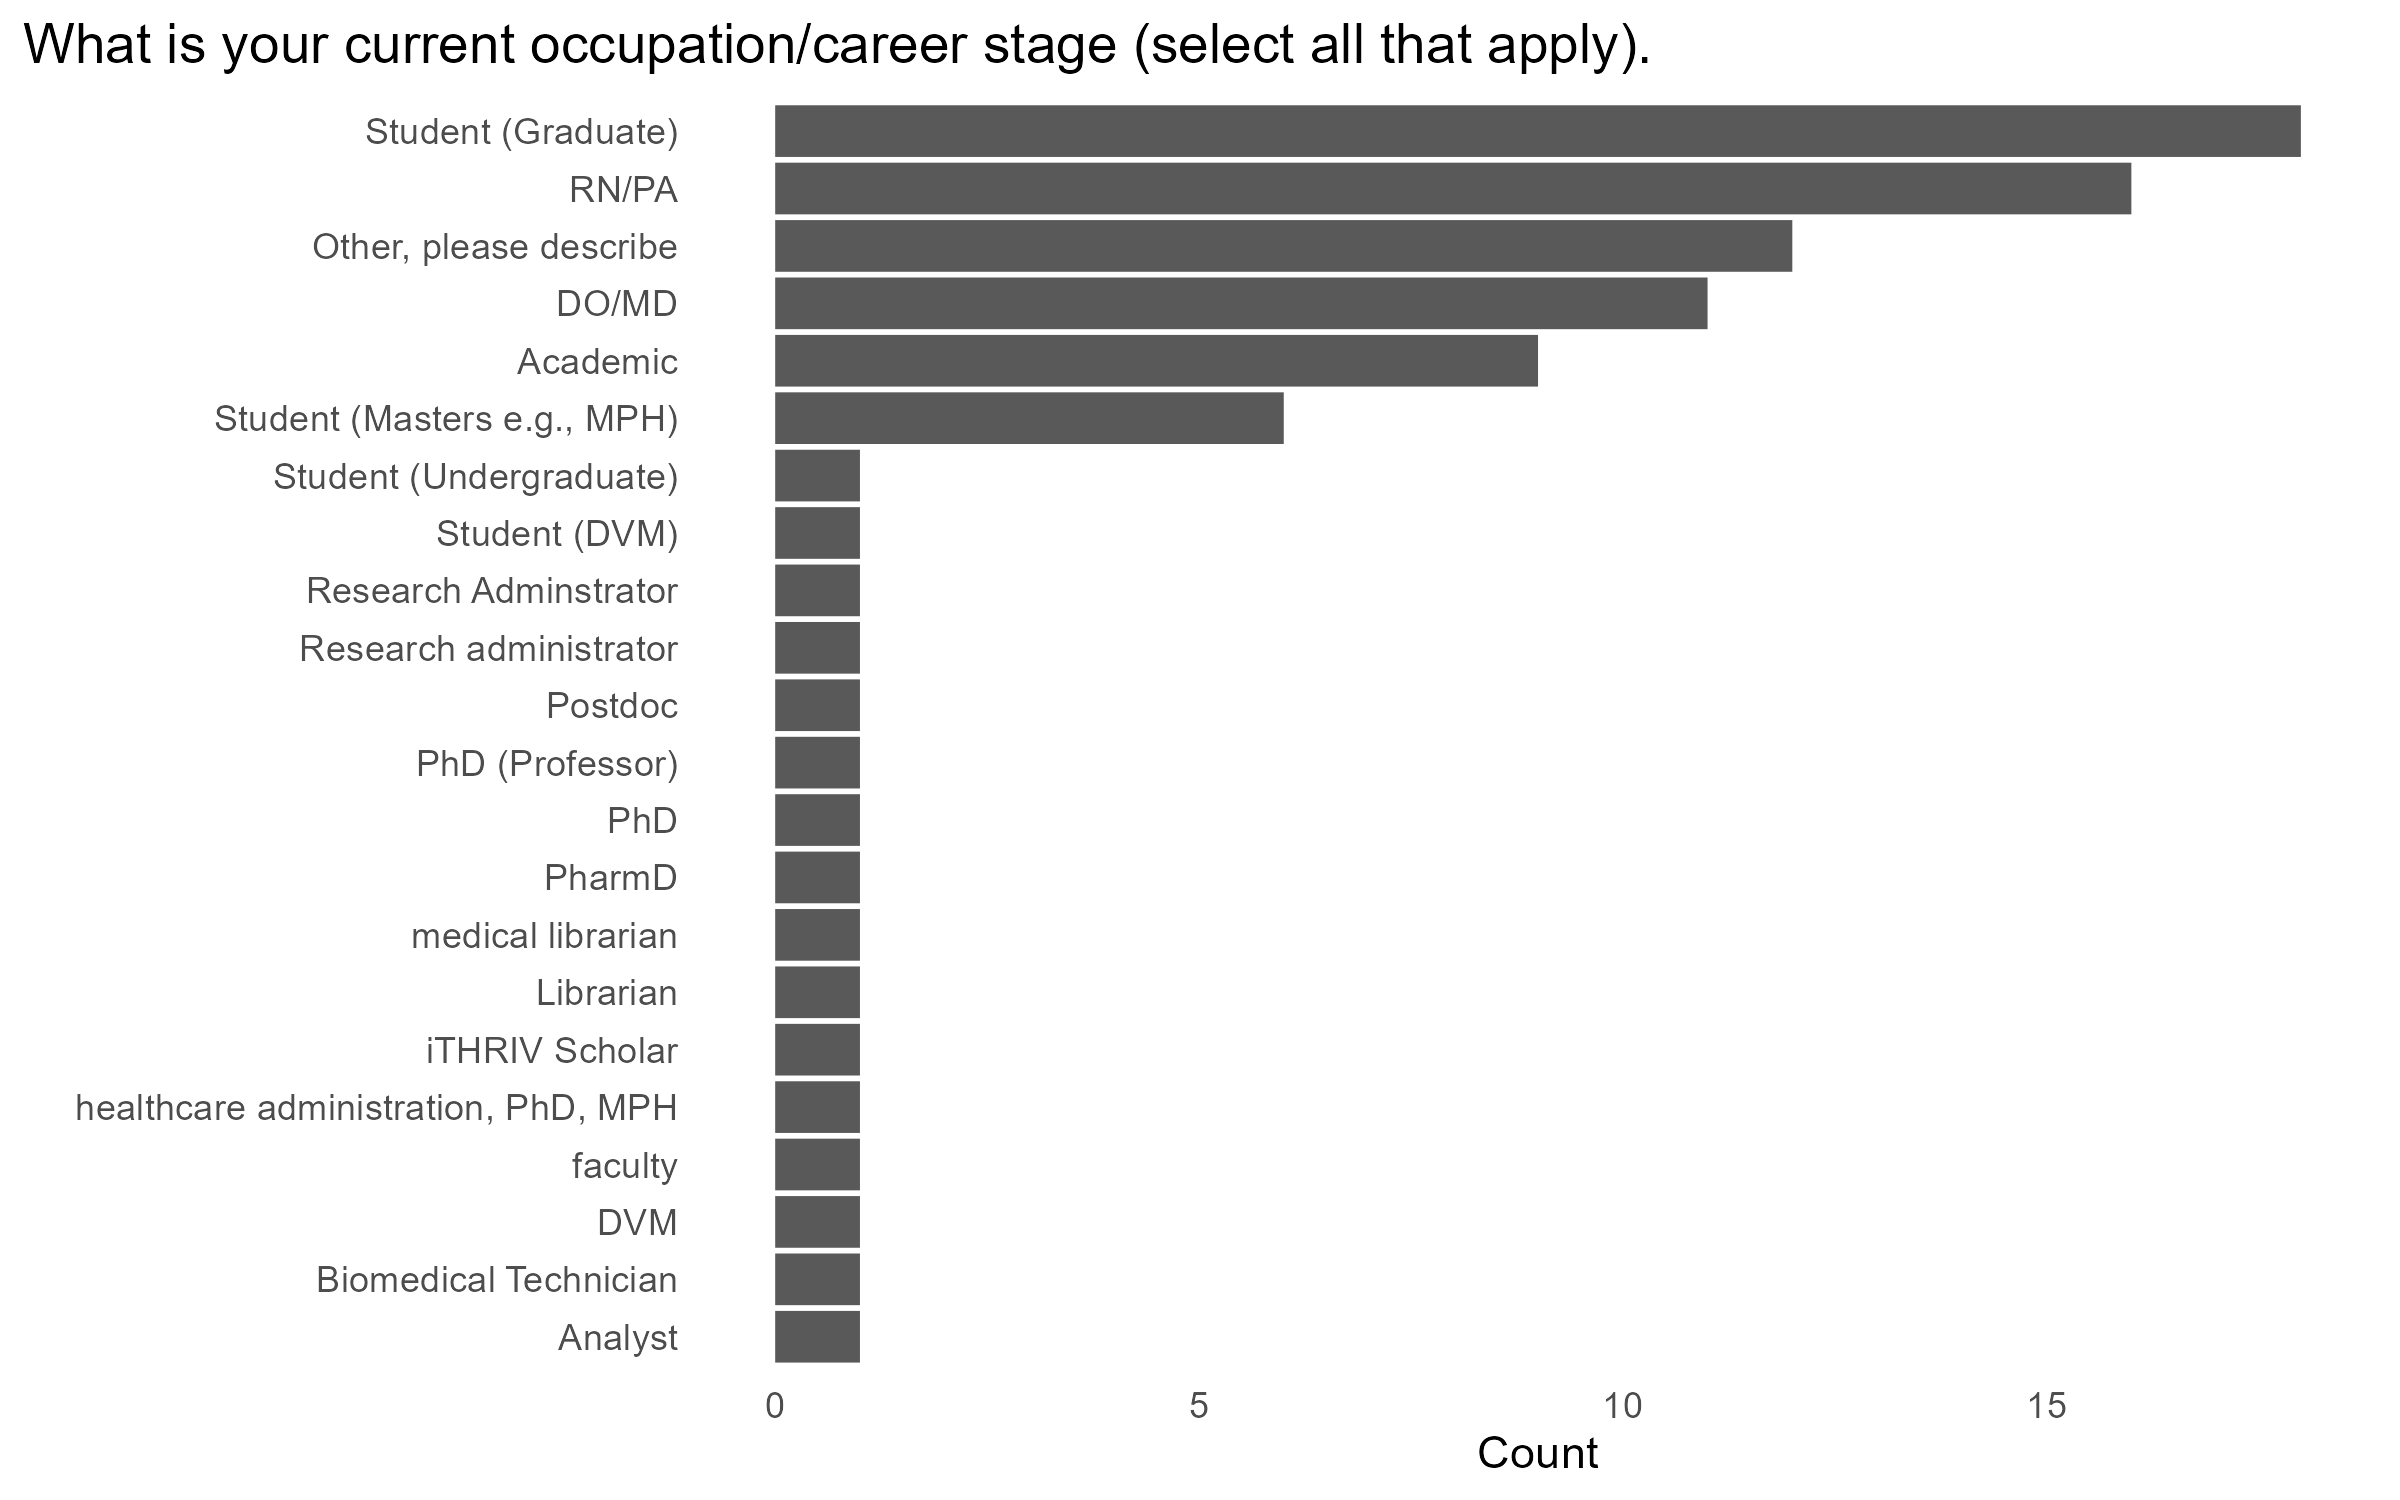
\includegraphics[width=0.7\linewidth]{figs/020-persona/Q2.3.png}
        \caption[What is your current occupation/career stage (select all that apply)]
        {Self reported current occupation and career stage.
            Respondents are able to select multiple options and also write in their own choices.
        }
        \label{fig:demographics_occupation}
    \end{figure}

    \begin{figure}[htb]
        \centering
        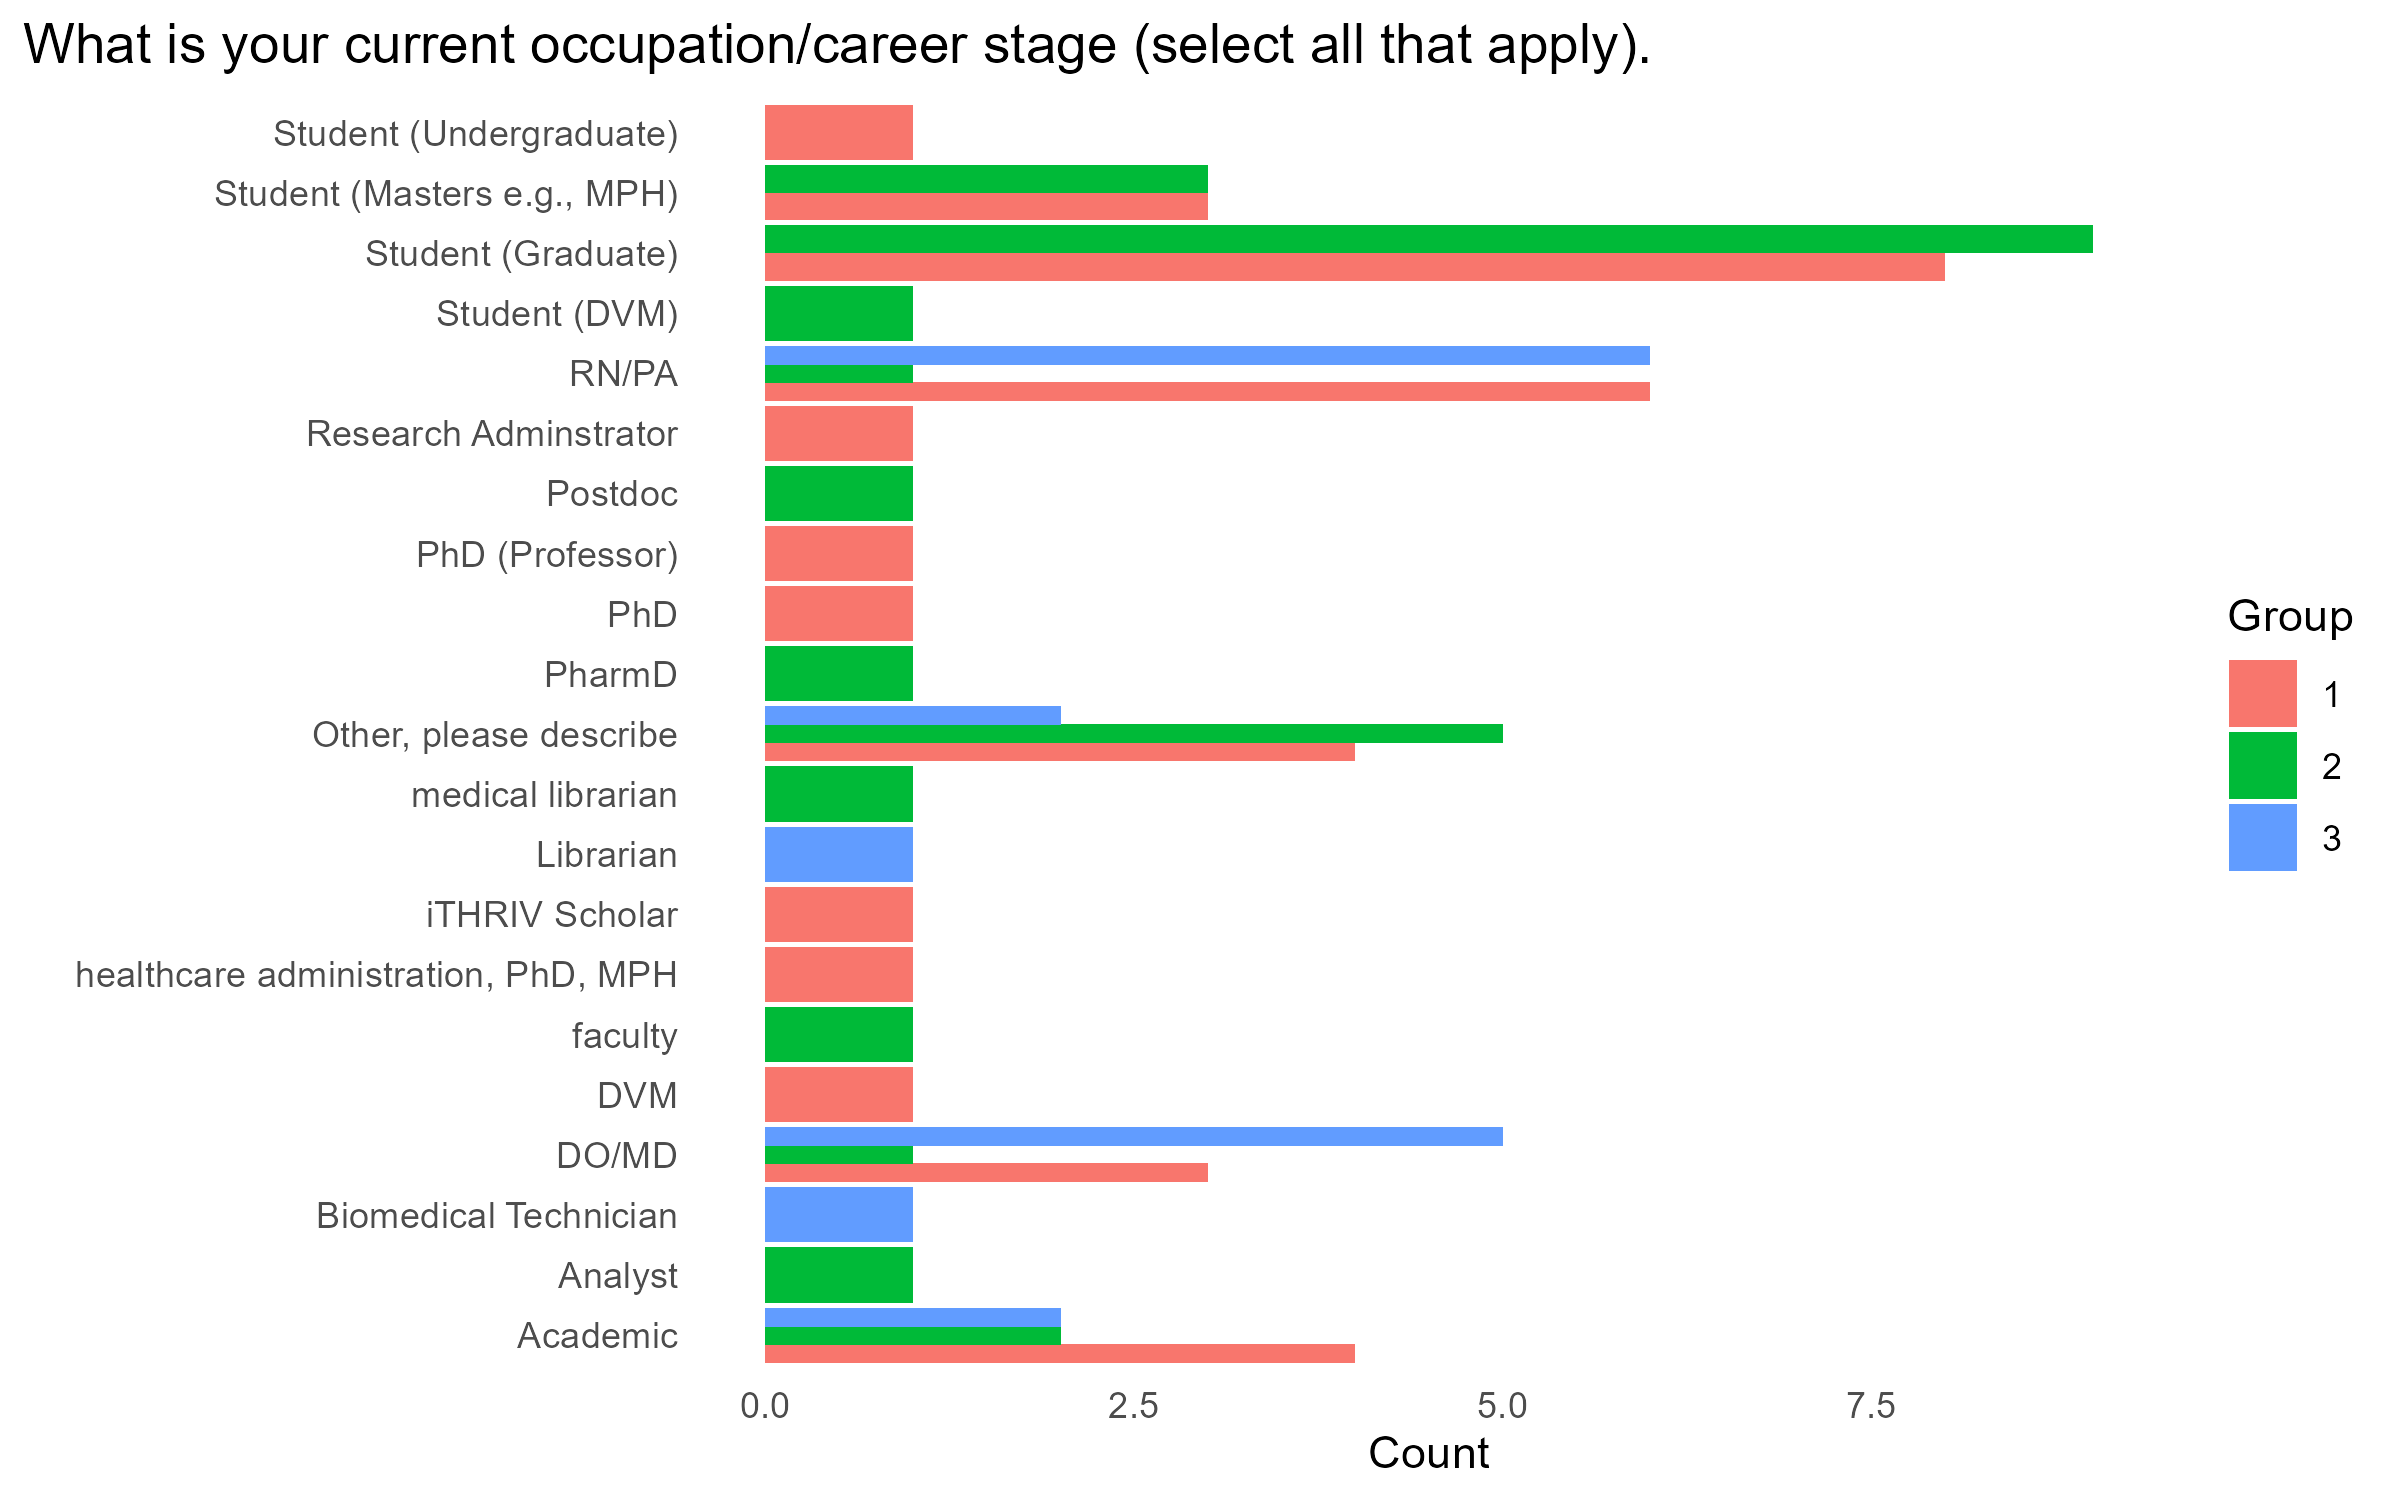
\includegraphics[width=0.7\linewidth]{figs/020-persona/survey\_likert/Q2.3-group-3.png}
        \caption[What is your current occupation/career stage by group (select all that apply)]
        {Self reported current occupation and career stage by clustering group.
            Respondents are able to select multiple options and also write in their own choices.
        }
        \label{fig:demographics_occupation_cluster}
    \end{figure}

    \begin{figure}[htb]
        \centering
        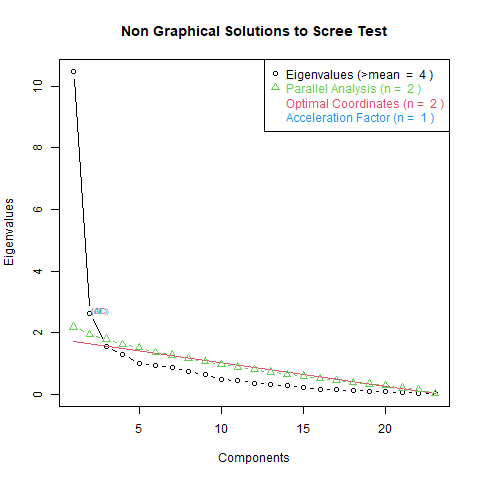
\includegraphics[scale=0.5]{figs/010-validation/efa_eigen_scree.png}
        \caption[Scree plot for factor analysis]
        {Scree plot for factor analysis showing the number of components (x) and the eigenvalues (y) for all 23 survey items.
            The figure suggests exploring 2 to 4 factor models.
        }
        \label{fig:scree-fa-all}
    \end{figure}



\end{document}
